\documentclass[12pt,a4paper,twoside,openright]{report}
\usepackage{setspace} % importowanie pakietu do ustawiania interlinii
\onehalfspacing % ustawienie interlinii 1.5
\usepackage{tgtermes}
\usepackage[T1]{fontenc}
\usepackage{polski}
\usepackage[utf8]{inputenc}
\input glyphtounicode
\pdfgentounicode=1
\usepackage{amssymb}
\usepackage{amsmath}
\usepackage{float}
\usepackage{pgfplots}
\usepackage{titlesec}
\usepackage{pgf-pie}
\usepackage{floatrow}
\usepackage{sectsty}
\usepackage{placeins}
\usepackage{pdfpages}
\usepackage{csquotes}
\usepackage{graphicx}
\usepackage{caption}
\let\lll\undefined
\usepackage{indentfirst}
\usepackage{float}
\usepackage{tabularx}
\usepackage{hyperref}
\graphicspath{ {./img/} }
\usepackage[left=2.5cm,right=2.5cm,top=2.5cm,bottom=2.5cm]{geometry}
\usepackage{caption}
\captionsetup{font=small}

\newcommand{\mycaption}[2]{%
  \caption[#1]{#1\\ \footnotesize{#2}}%
}
\usepackage{listings,lipsum}
\lstnewenvironment{myverbatim}[1][]{%
  \lstset{
    basicstyle=\ttfamily,
    frame=tb,
    #1
  }%
}{}
\usepackage{tocloft}
\usepackage{etoolbox}
\usepackage{datetime}
\usepackage{dirtree}
\renewcommand\DTstyle{\rmfamily}
\usepackage{listings}
\usepackage{titlesec}
\usepackage[defernumbers=true,
        locallabelwidth,
        backend=biber]{biblatex}

\pretocmd{\chapter}{\addtocontents{toc}{\protect\addvspace{-5pt}}}{}{}

\newcommand*{\typeprefix}{%
  \ifentrytype{article}{%%
  }{%
    \ifentrytype{book}{%%
    }{%
      www. % "other"
    }%
  }%
}

\DeclareFieldFormat{labelnumber}{\typeprefix #1}
\renewcommand*{\finentrypunct}{}

\lstset{
	basicstyle=\footnotesize\ttfamily,
    keepspaces=true,
    showstringspaces=false,
    commentstyle=\ttfamily,
    frame=single,
    aboveskip=18pt,
    belowskip=18pt,
    breaklines=true,
}
\raggedbottom
\usepackage[justification=centering]{caption}
\makeatletter
% \def\@makechapterhead#1{%
% \pagebreak
%   \vspace*{120\p@}% <----------------- Space from top of page to Chapter #
%   {\parindent \z@ \raggedright
%     \ifnum \c@secnumdepth >\m@ne
%         \huge\bfseries \@chapapp\space \thechapter. \Huge \bfseries #1\par\nobreak% <-- Chapter #
%         \par\nobreak
%         \vskip 24\p@% <-------------- Space between Chapter # and title
%   }}

\titlespacing{\section}{0pt}{12pt}{6pt}
\titlespacing{\subsection}{0pt}{6pt}{6pt}
\titlespacing{\footnotesize}{0pt}{10pt}
% Ustawienie domyślnej wielkości czcionki dla sekcji na 13pt
\makeatletter
\renewcommand{\section}{\@startsection{section}{1}{0mm}{\baselineskip}{0.5\baselineskip}{\normalfont\fontsize{13}{15}\bfseries}}
\makeatother
% Ustawienie domyślnej wielkości czcionki dla tabel na 13pt
\AtBeginEnvironment{tabular}{\fontsize{10}{10}\selectfont}
\preto\tabular{\centering}
 % Formatowanie chaptera
\makeatletter
\def\@makechapterhead#1{%
  \vspace*{12\p@}% 
  {\parindent \z@ \raggedright \normalfont
    \ifnum \c@secnumdepth >\m@ne
        \fontsize{14pt}{18pt}\bfseries \@chapapp\space \thechapter.\space #1\par\nobreak
        \vskip 20\p@
    \fi
    \interlinepenalty\@M
    \vskip 6\p@ 
  }}
\makeatother


\author{Kamil Piech}
\linespread{1.5}
\let\cleardoublepage=\clearpage

\renewcommand\cftchapfont{\fontsize{12pt}{18pt}\bfseries}
\renewcommand\cftsecfont{\fontsize{12pt}{18pt}}
\renewcommand\cftchappagefont{\fontsize{12pt}{18pt}\bfseries}
\renewcommand\cftsecpagefont{\fontsize{12pt}{18pt}}
\renewcommand{\cfttoctitlefont}{\vspace{-1.5cm}\fontsize{14pt}{}\bfseries}

\begin{document}
\captionsetup{font=footnotesize}
    \begin{titlepage}
    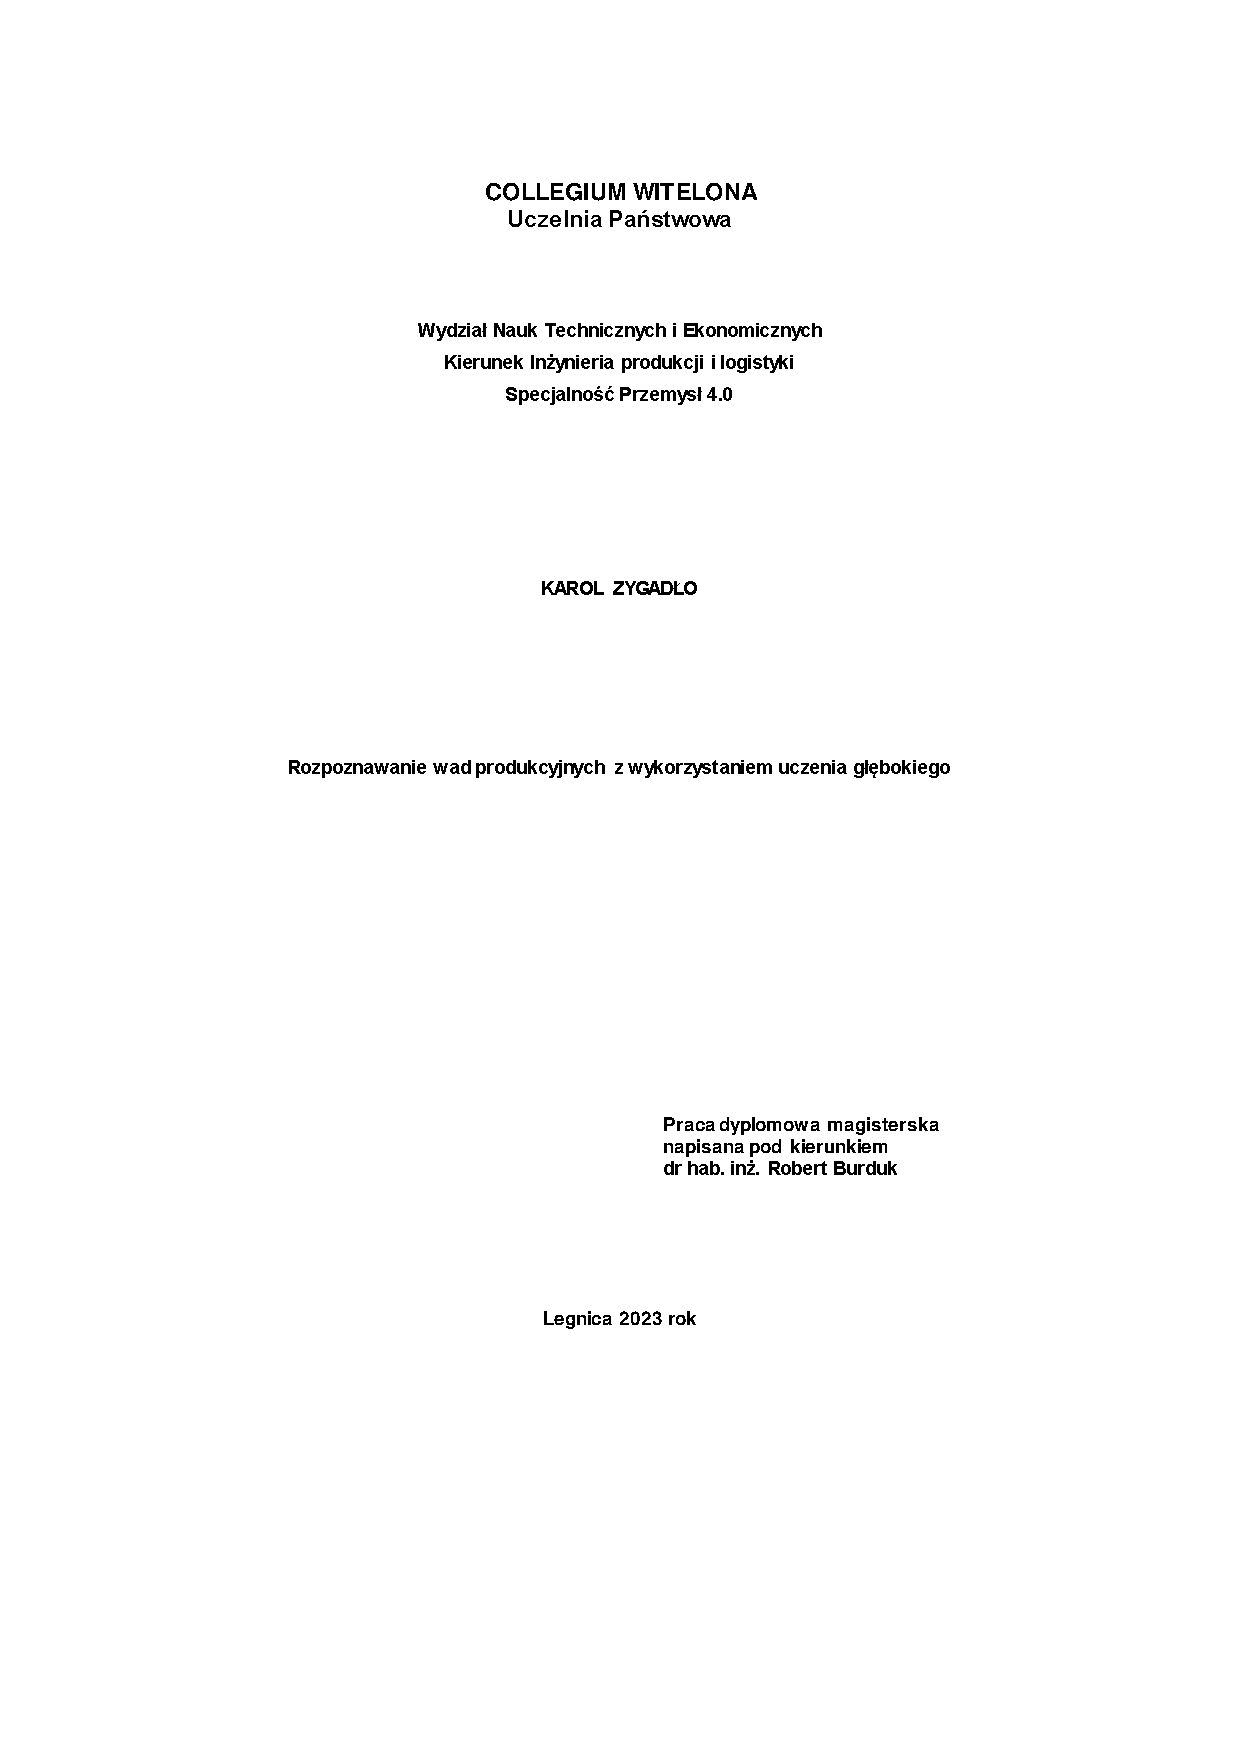
\includepdf{TitlePage.pdf}
    \end{titlepage}
    \tableofcontents
\begingroup
\setlength{\parindent}{0.7cm}

    % \let\clearpage\relax
    \chapter{Wstęp}
\section{Cel i motywacja pracy}

Celem niniejszej pracy magisterskiej jest opracowanie i zastosowanie metod uczenia głębokiego w celu rozpoznawania wad produkcyjnych na podstawie analizy zdjęć. Ze względu na coraz większe zapotrzebowanie na szybkie i efektywne rozwiązania w zakresie kontroli jakości, zastosowanie technik sztucznej inteligencji staje się niezbędne dla przemysłu. W szczególności, wykorzystanie uczenia głębokiego, jako jednego z najbardziej zaawansowanych podejść w dziedzinie sztucznej inteligencji, pozwala na znaczące zwiększenie skuteczności wykrywania wad produkcyjnych.

Motywacją do podjęcia tego tematu była chęć eksploracji i zrozumienia nowoczesnych technologii związanych z uczeniem maszynowym oraz ich praktyczne zastosowanie w kontekście przemysłowym. Wadliwe komponenty mogą prowadzić do znacznych strat finansowych oraz wpływać negatywnie na reputację przedsiębiorstwa. Automatyczne wykrywanie wad na wczesnym etapie procesu produkcyjnego może przyczynić się do zwiększenia efektywności, zmniejszenia kosztów oraz ograniczenia ilości produktów o niskiej jakości trafiających do odbiorców.

W ramach pracy magisterskiej opracowany zostanie system, który będzie w stanie analizować zdjęcia przedmiotów i automatycznie klasyfikować je jako wadliwe lub prawidłowe. System ten będzie oparty na technikach uczenia głębokiego, takich jak konwolucyjne sieci neuronowe, które są obecnie szeroko stosowane w różnych dziedzinach analizy obrazów. Praca będzie obejmować zarówno teorię, jak i praktyczne aspekty projektowania, implementacji oraz oceny tego rodzaju systemów.

W celu zilustrowania koncepcji i metod przedstawionych w pracy, zostanie przeprowadzone eksperymentalne zastosowanie opracowanego systemu do wybranego zbioru zdjęć reprezentujących obiekty z wadami produkcyjnymi oraz prawidłowymi komponentami. Wyniki tego eksperymentu posłużą jako dowód na skuteczność zastosowanego podejścia oraz jako punkt wyjścia do dalszej dyskusji na temat potencjalnych ulepszeń i przyszłych kierunków rozwoju.

\section{Zawartość pracy}

W niniejszej pracy dyplomowej skupiamy się na zagadnieniu wykrywania wad produkcyjnych z wykorzystaniem uczenia głębokiego, w szczególności sieci konwolucyjnych. Zakres pracy obejmuje następujące aspekty:

\begin{itemize}
\item Zaprezentowanie wybranych podstaw teoretycznych związanych z uczeniem głębokim, sieciami konwolucyjnymi oraz ich zastosowaniem w przemyśle;
\item Analiza istniejących rozwiązań i technologii stosowanych w kontroli jakości, w tym systemów wizyjnych, Internetu Rzeczy (IoT) oraz analizy danych;
\item Opracowanie projektu systemu, który spełnia określone wymagania funkcjonalne i niefunkcjonalne, oraz omówienie kroków projektowania takich jak wybór sieci konwolucyjnej, wczytywanie danych czy wstępne przetwarzanie danych;
\item Implementacja algorytmu uczenia głębokiego na podstawie opracowanego projektu, przedstawienie budowy modelu sieci neuronowej oraz etapów trenowania i testowania modelu;
\item Ewaluacja i analiza wyników uzyskanych podczas testów skuteczności i wydajności opracowanego systemu;
\item Prezentacja działania programu na przykładach zastosowań;
\item Podsumowanie wyników pracy, wskazanie zrealizowanych celów oraz przedstawienie perspektyw na dalsze badania i rozwój systemu.
\end{itemize}

W ramach pracy został opracowany kod źródłowy, który prezentuje implementację modelu sieci neuronowej oraz wszystkie etapy przetwarzania danych, trenowania, testowania i ewaluacji modelu. Kod źródłowy został napisany w wybranym języku programowania i korzysta z odpowiednich bibliotek oraz narzędzi dedykowanych dla uczenia głębokiego i sieci konwolucyjnych.
    \chapter{Wybrane podstawy teoretyczne pracy}

\section{Uczenie głębokie}
Uczenie głębokie to gałąź uczenia maszynowego, która skupia się na zastosowaniu sztucznych sieci neuronowych z wieloma warstwami ukrytymi. W przeciwieństwie do tradycyjnych metod uczenia maszynowego, takich jak regresja liniowa czy drzewa decyzyjne, uczenie głębokie automatycznie odkrywa reprezentacje danych na różnych poziomach abstrakcji. Jest to kluczowe dla rozwiązywania złożonych problemów, takich jak rozpoznawanie obrazów, przetwarzanie języka naturalnego, rozpoznawanie mowy czy analiza danych biologicznych.

\subsection{Historia uczenia głębokiego}
Historia uczenia głębokiego sięga lat 40. XX wieku, kiedy to badacze zaczęli eksplorować koncepcje sztucznych neuronów, które próbowały naśladować biologiczne procesy zachodzące w ludzkim mózgu. W 1986 roku Rumelhart, Hinton i Williams wprowadzili algorytm wstecznej propagacji błędów (backpropagation), który umożliwił efektywne uczenie się sieci neuronowych.

W 2006 roku Hinton i Salakhutdinov opublikowali pracę, która przyczyniła się do powstania współczesnego uczenia głębokiego. Przedstawili w niej skonstruowane przez siebie głębokie sieci wstępnie uczące się (deep belief networks) i pokazali, że sieci te potrafią uczyć się reprezentacji danych na wielu poziomach abstrakcji. Od tego czasu uczenie głębokie zyskało na popularności, a rozwój technologii przyczynił się do udoskonalenia algorytmów oraz wykorzystania uczenia głębokiego w praktyce.

\subsection{Zastosowania uczenia głębokiego}
Uczenie głębokie znalazło szerokie zastosowanie w różnych dziedzinach nauki i przemysłu. Przykłady obejmują:
\begin{itemize}
\item Rozpoznawanie obrazów: wykorzystanie sieci konwolucyjnych (CNN) do klasyfikacji obrazów, detekcji obiektów czy segmentacji obrazów.
\item Przetwarzanie języka naturalnego: stosowanie rekurencyjnych sieci neuronowych (RNN) i mechanizmów uwagi (attention) do tłumaczenia maszynowego, generowania tekstu czy analizy uczuć.
\item Rozpoznawanie mowy: zastosowanie sieci neuronowych do rozpoznawania mowy i konwersji mowy na tekst.
\item Wzmocnienie ucznia: wykorzystanie uczenia głębokiego w połączeniu z algorytmami uczenia przez wzmacnianie do sterowania robotami, pojazdami autonomicznymi czy strategiami giełdowymi.
\end{itemize}

\subsection{Różnice między uczeniem głębokim a innymi technikami uczenia maszynowego}
Uczenie głębokie różni się od innych technik uczenia maszynowego w kilku kluczowych aspektach:

\begin{itemize}
\item \textbf{Reprezentacja danych:} Uczenie głębokie automatycznie uczy się reprezentacji danych na różnych poziomach abstrakcji, podczas gdy w tradycyjnych metodach uczenia maszynowego, takich jak SVM czy drzewa decyzyjne, inżynierowie muszą ręcznie projektować cechy (feature engineering), które mają być użyte do uczenia modelu.
\item \textbf{Architektura sieci:} Sieci neuronowe stosowane w uczeniu głębokim mają wiele warstw ukrytych, co pozwala na uczenie się bardziej złożonych funkcji. W przeciwnym razie, metody uczenia maszynowego często korzystają z modeli o mniejszej złożoności, takich jak regresja liniowa czy drzewa decyzyjne.
\item \textbf{Skalowalność:} Dzięki efektywnym algorytmom optymalizacji oraz rosnącej mocy obliczeniowej, uczenie głębokie może być stosowane do przetwarzania ogromnych zbiorów danych. W porównaniu, inne techniki uczenia maszynowego mają trudności z działaniem na dużą skalę, szczególnie gdy wymagane jest ekstrahowanie cech z dużych zbiorów danych.
\item \textbf{Transfer wiedzy:} W uczeniu głębokim istnieje możliwość wykorzystania wiedzy uzyskanej z jednego zadania do innych zadań, co jest nazywane uczeniem transferowym (transfer learning). W tradycyjnym uczeniu maszynowym transfer wiedzy jest trudniejszy do osiągnięcia.
\end{itemize}

\section{Sieci konwolucyjne}
Sieci konwolucyjne (CNN) to specjalny rodzaj sieci neuronowych, w których zastosowano warstwy konwolucyjne. Warstwy te analizują obrazy za pomocą filtrów, które są przesuwane po danych wejściowych, generując mapy cech. Filtry te uczą się wykrywać lokalne wzorce, takie jak krawędzie, tekstury czy kształty. Warstwy pooling (agregujące) są stosowane w celu zmniejszenia wymiarowości map cech, co prowadzi do redukcji ilości parametrów w sieci. Sieci konwolucyjne mogą być również wykorzystywane w połączeniu z innymi warstwami, takimi jak warstwy gęsto połączone (fully connected) czy rekurencyjne (RNN), w zależności od problemu, który mają rozwiązać.

\subsection{Wady produkcyjne i ich rodzaje}
Wady produkcyjne to niezgodności w produkcji, które powodują, że produkt nie spełnia swoich wymagań jakościowych. Mogą być spowodowane przez wiele czynników, takich jak nieprawidłowości w procesie produkcyjnym, zużycie maszyn czy błędy ludzkie. Wady produkcyjne można podzielić na różne rodzaje, w zależności od charakterystyki produktu i procesu produkcyjnego. Niektóre z najbardziej powszechnych rodzajów wad produkcyjnych obejmują:

\begin{itemize}
\item \textbf{Wady powierzchniowe:} Pęknięcia, zadrapania, zmarszczki, przebarwienia czy zanieczyszczenia na powierzchni produktu.
\item \textbf{Wady geometryczne:} Niewłaściwe wymiary, kształty czy położenie elementów w stosunku do siebie nawzajem.
\item \textbf{Wady materiałowe:} Wady w strukturze materiału, takie jak pęcherze powietrza, porowatość czy zanieczyszczenia.
\item \textbf{Wady funkcjonalne:} Problemy z działaniem produktu wynikające z nieprawidłowego montażu, błędów w projektowaniu czy wadliwych komponentów.
\end{itemize}

\subsection{Istniejące rozwiązania}
W przemyśle istnieje wiele rozwiązań do wykrywania wad produkcyjnych. Tradycyjne metody obejmują wizualne sprawdzanie produktów przez operatorów, które może być czasochłonne i podatne na błędy. Inne metody obejmują stosowanie systemów wizyjnych z kamerami i algorytmami przetwarzania obrazów, które analizują produkty pod kątem wad. Te metody jednak często wymagają ręcznego projektowania cech oraz są trudne do skalowania.

Uczenie głębokie, a w szczególności sieci konwolucyjne, oferuje nowe możliwości w zakresie wykrywania wad produkcyjnych. Dzięki automatycznemu uczeniu się reprezentacji danych, sieci konwolucyjne potrafią wykrywać wady na obrazach z wysoką precyzją i są łatwe do skalowania. Ponadto, uczenie transferowe pozwala na zastosowanie wiedzy uzyskanej z jednego zadania do innego, co ułatwia adaptację modeli do różnych rodzajów wad i procesów produkcyjnych.

\subsection{Wybrane języki programowania}
\subsubsection{Python}
Python to popularny język programowania o otwartym kodzie źródłowym, który cechuje się prostotą, czytelnością i wszechstronnością. Jest szeroko stosowany w uczeniu maszynowym i uczeniu głębokim dzięki bogatemu ekosystemowi bibliotek, takich jak TensorFlow, PyTorch czy scikit-learn. Python oferuje wiele narzędzi do analizy danych, wizualizacji, pracy z obrazami i dźwię

    \chapter{Projekt systemu}
\section{Wymagania}
\section{Projekt rozwiązania}
\subsection{Import bibliotek}
\subsection{Wczytywanie danych}
\subsection{Przygotowanie danych do uczenia}
\subsection{Podział danych na zestawy treningowe, walidacyjne i testowe}
    \chapter{Implementacja}
\section{Budowa modelu sieci neuronowej}

W celu rozwiązania problemu rozpoznawania wad produkcyjnych, zastosowano sieć neuronową opartą na architekturze konwolucyjnej (CNN). Sieci tego typu są powszechnie używane w problemach analizy obrazów, ponieważ potrafią efektywnie wykrywać lokalne wzorce i cechy na obrazach. W tym przypadku, sieć będzie w stanie nauczyć się rozpoznawania różnych wad produkcyjnych na podstawie analizy dostarczonych zdjęć.

Model sieci neuronowej został zaimplementowany przy użyciu biblioteki TensorFlow w języku Python. Poniżej przedstawiono kod źródłowy użyty do budowy modelu:

\begin{verbatim}
from tensorflow.keras.models import Sequential
from tensorflow.keras.layers import Conv2D, MaxPooling2D, Dense, Flatten, Dropout

model = Sequential()

model.add(Conv2D(16, (3,3), 1, activation='relu', input_shape=(256,256,3)))
model.add(MaxPooling2D())

model.add(Conv2D(32, (3,3), 1, activation='relu'))
model.add(MaxPooling2D())

model.add(Conv2D(16, (3,3), 1, activation='relu'))
model.add(MaxPooling2D())

model.add(Flatten())
model.add(Dense(256, activation='relu'))
model.add(Dense(1, activation='sigmoid'))
\end{verbatim}

Sieć składa się z trzech warstw konwolucyjnych z funkcją aktywacji ReLU oraz warstwami MaxPooling po każdej z nich. Warstwy konwolucyjne uczą się wykrywać lokalne cechy na obrazach, a MaxPooling pomaga w redukcji wymiarowości, co przyspiesza uczenie i zmniejsza ryzyko przeuczenia.

Po trzech warstwach konwolucyjnych, sieć przechodzi przez warstwę Flatten, która spłaszcza dane do jednowymiarowego wektora, co pozwala na przekazanie ich do warstw gęstych (Dense). W tym przypadku, użyto jednej warstwy gęstej z 256 neuronami i funkcją aktywacji ReLU.

Na końcu, sieć kończy się warstwą gęstą z jednym neuronem i funkcją aktywacji sigmoidalną. Ta warstwa odpowiada za generowanie wyników klasyfikacji, gdzie wartość bliska 0 wskazuje na uszkodzony produkt, a wartość bliska 1 na prawidłowy.

Model został skompilowany z użyciem optymalizatora Adam, funkcji straty BinaryCrossentropy oraz metryki dokładności:

\begin{verbatim}
model.compile('adam', loss=tf.losses.BinaryCrossentropy(),
metrics=['accuracy'])
\end{verbatim}

Zastosowanie optymalizatora Adam pomaga w szybszym i skuteczniejszym uczeniu się sieci, gdyż dostosowuje szybkość uczenia na podstawie zmian gradientu. Funkcja straty BinaryCrossentropy jest odpowiednia do problemów klasyfikacji binarnej, takich jak ten, ponieważ pozwala na ocenę różnic między prawdziwymi etykietami a prognozowanymi przez sieć.

\section{Trenowanie modelu}

Trenowanie modelu sieci neuronowej to proces optymalizacji wag w sieci, aby osiągnąć jak najlepszą wydajność w rozpoznawaniu wad produkcyjnych na podstawie zdjęć. W implementacji wykorzystano dane treningowe i walidacyjne do uczenia modelu oraz oceny jego wydajności podczas trenowania. W tej sekcji omówione zostanie trenowanie modelu, analiza wydajności oraz sposób monitorowania procesu uczenia.

Wykorzystano metodę \verb|fit| dostarczoną przez bibliotekę Keras, aby przeszkolić model sieci neuronowej. Poniższy kod przedstawia sposób trenowania modelu przez 5 epok, używając danych treningowych oraz walidacyjnych:

\begin{verbatim}
hist = model.fit(train, epochs=5, validation_data=val, callbacks=[tensorboard_callback])
\end{verbatim}

Parametr \verb|epochs| określa liczbę pełnych przebiegów przez dane treningowe. W każdej epoce model próbuje zminimalizować funkcję straty na danych treningowych, dostosowując wagi sieci neuronowej. Użycie danych walidacyjnych pozwala na obserwację procesu uczenia się i wykrycie ewentualnego przeuczenia modelu. Jeśli model zaczyna się przeuczać, dokładność na danych walidacyjnych zacznie maleć, podczas gdy dokładność na danych treningowych nadal będzie rosnąć.

TensorBoard to narzędzie do wizualizacji uczenia sieci neuronowych, które pozwala na monitorowanie różnych metryk, takich jak funkcja straty i dokładność. W implementacji użyto TensorBoard jako wywołania zwrotnego (ang. callback) podczas trenowania, co pozwala na automatyczne zapisywanie danych do logów:

\begin{verbatim}
logdir='logs'
tensorboard_callback = tf.keras.callbacks.TensorBoard(log_dir=logdir)
\end{verbatim}

Logi TensorBoard można następnie wyświetlić w przeglądarce, aby uzyskać interaktywną wizualizację procesu uczenia. Aby uruchomić TensorBoard, należy wpisać w terminalu poniższe polecenie, a następnie otworzyć wyświetlony adres URL w przeglądarce:

\begin{verbatim}
tensorboard --logdir=logs
\end{verbatim}

Po zakończeniu trenowania modelu, można ocenić jego wydajność na podstawie historii uczenia. Poniższy kod przedstawia sposób tworzenia wykresów straty oraz dokładności dla danych treningowych i walidacyjnych:

\begin{verbatim}
fig = plt.figure()
plt.plot(hist.history['loss'], color='teal', label='strata treningowa')
plt.plot(hist.history['val_loss'], color='orange', label='strata walidacji')
fig.suptitle('Strata', fontsize=20)
plt.legend(loc="upper left")
plt.show()

fig = plt.figure()
plt.plot(hist.history['accuracy'], color='teal', label='dokładność treningowa')
plt.plot(hist.history['val_accuracy'], color='orange', label='dokładność walidacji')
fig.suptitle('Dokładność', fontsize=20)
plt.legend(loc="upper left")
plt.show()
\end{verbatim}

Wykresy te pozwalają na analizę wydajności modelu w czasie trenowania. Na wykresie straty obserwujemy spadek wartości funkcji straty zarówno dla danych treningowych, jak i walidacyjnych. Jeśli model jest odpowiednio uczone, strata na danych walidacyjnych powinna stabilizować się na niskim poziomie.

Wykres dokładności przedstawia, jak dobrze model radzi sobie z klasyfikacją próbek na danych treningowych i walidacyjnych. W miarę jak model się uczy, dokładność powinna rosnąć, aż osiągnie pewien poziom, po którym może wystąpić przeuczenie. W przypadku przeuczenia, dokładność na danych treningowych będzie nadal rosnąć, podczas gdy dokładność na danych walidacyjnych będzie maleć.

Podsumowując, trenowanie modelu sieci neuronowej to proces uczenia modelu na danych treningowych oraz oceny jego wydajności na danych walidacyjnych. Użycie TensorBoard pozwala na monitorowanie tego procesu w czasie rzeczywistym, a analiza wykresów straty oraz dokładności pozwala na ocenę jakości uczenia modelu. Dostosowanie liczby epok oraz parametrów modelu może poprawić jego wydajność i ograniczyć przeuczenie.

\section{Ewaluacja modelu}
\section{Wizualizacja wyników}
\section{Testowanie modelu na przykładach}
\section{Zapis i odczyt modelu}
    \chapter{Badanie, porównanie efektywności systemu}
\section{Testy wydajności}
\section{Testy skuteczności}
\section{Analiza skuteczności}
    \chapter{Prezentacja działania programu}
    \chapter{Podsumowanie}
\section{Wnioski}
W wyniku przeprowadzonych badań można wysnuć następujące wnioski:

\begin{enumerate}
\item Liczba zdjęć użytych do wyuczenia modelu ma znaczący wpływ na jego dokładność w rozpoznawaniu wad produkcyjnych. Wraz ze wzrostem liczby zdjęć użytych do nauki, dokładność modelu zwykle się poprawia.
\item Model wyuczony na 500 zdjęciach osiągnął najwyższą dokładność w testach, co sugeruje, że większa liczba danych uczących przyczynia się do lepszej generalizacji modelu.
\item W przypadku małych zbiorów danych, model może być narażony na przetrenowanie, co skutkuje słabszymi wynikami na danych testowych.
\item Potrzeba dalszych badań nad optymalizacją architektury modelu oraz eksploracją innych technik przetwarzania wstępnego danych, takich jak augmentacja danych, aby poprawić wydajność modelu.
\item Zastosowanie różnych technik uczenia transferowego może przyczynić się do zwiększenia skuteczności modelu, szczególnie w przypadku mniejszych zbiorów danych.
\end{enumerate}

W oparciu o przeprowadzone badania, można zidentyfikować następujące kierunki dalszego rozwoju projektu:

\begin{itemize}
\item Eksploracja innych architektur sieci głębokiego uczenia, takich jak sieci ResNet, DenseNet lub Inception, które mogą osiągać lepsze wyniki w rozpoznawaniu wad produkcyjnych.
\item Zastosowanie technik augmentacji danych, aby zwiększyć liczbę dostępnych danych uczących oraz poprawić generalizację modelu.
\item Implementacja mechanizmów regularyzacji, takich jak dropout, aby zmniejszyć ryzyko przetrenowania modelu, zwłaszcza w przypadku małych zbiorów danych.
\item Analiza wpływu różnych parametrów uczenia, takich jak rozmiar wsadu, współczynnik uczenia czy optymalizator, na dokładność modelu.
\item Badanie zastosowania uczenia transferowego, wykorzystując wytrenowane na dużych zbiorach danych modele do ekstrakcji cech, co może skrócić czas uczenia oraz poprawić skuteczność modelu na mniejszych zbiorach danych.
\item Eksploracja zastosowań modelu w innych dziedzinach, takich jak analiza jakości innych produktów, gdzie istnieje potrzeba wykrywania wad na podstawie zdjęć.
\end{itemize}

W kontekście praktycznym, wyniki badań oraz analizy mogą być wykorzystane do planowania i implementacji systemów kontroli jakości w różnych gałęziach przemysłu. Poprawa wydajności modelu w wykrywaniu wad produkcyjnych może przyczynić się do redukcji kosztów związanych z wadliwymi produktami oraz poprawy ogólnej jakości oferowanych produktów. W dłuższej perspektywie, opracowanie efektywnego i dokładnego modelu rozpoznawania wad może także pomóc w automatyzacji procesów kontroli jakości, co pozwoli na optymalizację zasobów i zwiększenie efektywności produkcji.

\section{Zrealizowane cele}

W ramach niniejszej pracy pt. "Rozpoznawanie wad produkcyjnych z wykorzystaniem uczenia głębokiego" osiągnięto szereg celów, które przyczyniły się do zrozumienia i wykorzystania technik uczenia głębokiego w celu wykrywania wad produkcyjnych. Poniżej przedstawiamy szczegółowy opis zrealizowanych celów:

\begin{itemize}
\item \textbf{Przegląd literatury :} Przeprowadzono obszerny przegląd literatury, który obejmował analizę podstawowych koncepcji uczenia głębokiego, sieci neuronowych, konwolucyjnych sieci neuronowych (CNN) oraz przegląd zastosowań tych technik w różnych dziedzinach przemysłu. Analiza literatury pozwoliła na zrozumienie podstawowych zagadnień związanych z uczeniem głębokim oraz na identyfikację kluczowych technik i metod, które mogą być wykorzystane w celu rozpoznawania wad produkcyjnych.
\item \textbf{Przygotowanie danych uczących}
Zebrano i przygotowano zbiór danych uczących, który obejmował zdjęcia przedstawiające produkty z wadami oraz produkty prawidłowe. Przeprowadzono wstępne przetwarzanie danych, takie jak skalowanie, kadrowanie i normalizację, aby ułatwić proces uczenia modelu. Przygotowanie odpowiedniego zbioru danych uczących stanowi podstawę dla późniejszego etapu uczenia modelu oraz oceny jego skuteczności.
\item \textbf{Budowa i uczenie modeli}
Zbudowano modele konwolucyjnych sieci neuronowych (CNN) z różnymi parametrami, takimi jak liczba warstw, rozmiar filtrów, funkcje aktywacji czy optymalizatory. Przeprowadzono uczenie modeli na różnych zbiorach danych uczących, obejmujących 25, 50, 100 oraz 500 zdjęć, co pozwoliło na analizę wpływu liczby danych uczących na skuteczność modelu.
\item \textbf{Ocena i analiza wyników}
Przeprowadzono testy modeli na danych testowych, które nie były wykorzystywane podczas uczenia. Analizowano skuteczność modeli na podstawie ich zdolności do poprawnego rozpoznawania produktów z wadami i produktów prawidłowych. Wyniki testów posłużyły do oceny ogólnej skuteczności modeli oraz do identyfikacji obszarów wymagających dalszych usprawnień.
\item \textbf{Wnioski i kierunki dalszego rozwoju}
Na podstawie przeprowadzonych badań sformułowano wnioski dotyczące zastosowania uczenia głębokiego w rozpoznawaniu wad produkcyjnych oraz zidentyfikowano kierunki dalszego rozwoju projektu. Wskazano między innymi, że liczba zdjęć użytych do wyuczenia modelu ma znaczący wpływ na jego dokładność, a model wyuczony na większej liczbie zdjęć osiąga lepsze wyniki. Zauważono również, że dalsze badania nad optymalizacją architektury modelu oraz eksploracją innych technik przetwarzania wstępnego danych mogą przyczynić się do poprawy wydajności modelu.
W ramach dalszego rozwoju projektu zidentyfikowano następujące kierunki:
\begin{itemize}
\item Eksploracja innych architektur sieci głębokiego uczenia, takich jak sieci ResNet, DenseNet lub Inception, które mogą osiągać lepsze wyniki w rozpoznawaniu wad produkcyjnych.
\item Zastosowanie technik augmentacji danych, aby zwiększyć liczbę dostępnych danych uczących oraz poprawić generalizację modelu.
\item Implementacja mechanizmów regularyzacji, takich jak dropout, aby zmniejszyć ryzyko przetrenowania modelu, zwłaszcza w przypadku małych zbiorów danych.
\item Analiza wpływu różnych parametrów uczenia, takich jak rozmiar wsadu, współczynnik uczenia czy optymalizator, na dokładność modelu.
\end{itemize}

\end{itemize}
\endgroup
\medskip

\renewcommand\bibname{\vspace{-2cm}\large{Bibliografia}}
\renewcommand\listfigurename{\vspace{-2cm}\large{Spis rysunków}}
\renewcommand\listtablename{\vspace{-2cm}\large{Spis tabel}}
\begin{thebibliography}{12} 
% \vspace{-1cm}
\bibitem{book} Yoshua Bengio, Ian Goodfellow, Aaron Courville, Deep Learning Systemy uczące się, Wydawnictwo Naukowe PWN, Warszawa, 2018.
\bibitem{book} Mariusz Flasiński, Wstęp do sztucznej inteligencji, Wydawnictwo Naukowe PWN, Warszawa, 2018.
\bibitem{book} Joel Grus, Data science od podstaw. Analiza danych w Pythonie, Helion, Gliwice, 2022.
\bibitem{book} Ryszard Knosala, Inżynieria produkcji, PWE Polskie Wydawnictwo Ekonomiczne, Warszawa 2017.
\bibitem{book} Robert A. Kosiński, Sztuczne sieci neuronowe, Wydawnictwo Naukowe PWN, Warszawa, 2017.
\bibitem{book} Yuxi Hayden Liu, Python Uczenie maszynowe w przykładach TensorFlow 2 PyTorch i scikitlearn, Helion, Gliwice, 2022.
\bibitem{book} Mark Lutz, Python. Wprowadzenie, Helion, Gliwice, 2022.
\bibitem{book} Sebastian Raschka, Vahid Mirjalili, Python Machine learning i deep learning, Helion, Gliwice, 2021.
\bibitem{book} Kazimierz Szatkowski, Nowoczesne zarządzanie produkcją, Wydawnictwo Naukowe PWN, Warszawa 2023.
\bibitem{book} Jerzy Surma, Hakowanie sztucznej inteligencji, Wydawnictwo Naukowe PWN, Warszawa, 2022.
\end{thebibliography}

\newpage
\listoffigures
\newpage
\listoftables

\newpage

\chapter*{}
\centering\textbf{OŚWIADCZENIE\\[6mm]}
\raggedright
Oświadczam, że: 
\begin{enumerate}
    \item pracę niniejszą przygotowałem(am) samodzielnie; wszystkie dane, istotne myśli i sformułowania pochodzące 
z literatury (przytoczone dosłownie lub niedosłownie) są opatrzone odpowiednimi odsyłaczami; praca ta nie była 
w całości ani w części przez nikogo przedkładana do żadnej oceny i nie była publikowana;
    \item wyrażam zgodę / nie wyrażam zgody na udostępnianie mojej pracy dyplomowej. 
\end{enumerate}\\[10mm]
Data ..............................\\[15mm]


\centering
\hspace{200pt} ..............................................\\[0mm]
\hspace{200pt} imię i nazwisko\\[10mm]
\hspace{200pt} Stwierdzam autentyczność podpisu\\[5mm]
\hspace{200pt} .....................................................................\\[0mm]
\hspace{200pt} (podpis  pracownika i pieczątka Wydziału)\\[20mm]
 
 \raggedright
 * niepotrzebne skreślić
\end{document}